\documentclass{article}

\PassOptionsToPackage{numbers,compress}{natbib}
\usepackage[preprint]{neurips_2023}

% The style file's preprint option prints "Preprint. Under review." This work is
% not under review anywhere, so the notice states only what is true.
\makeatletter
\renewcommand{\@noticestring}{Preprint.}
\makeatother

\usepackage[utf8]{inputenc}
\usepackage[T1]{fontenc}
\usepackage{hyperref}
\usepackage{url}
\usepackage{booktabs}
\usepackage{amsfonts}
\usepackage{amsmath}
\usepackage{nicefrac}
\usepackage{microtype}
\usepackage{graphicx}
\usepackage{xcolor}
\usepackage{longtable}

\hypersetup{colorlinks=true, linkcolor=black, citecolor=black, urlcolor=blue}

% Nine figures and ten tables against a twelve-page body will strand floats
% pages away from the text that references them unless the page is allowed to
% carry more of them.
\renewcommand{\topfraction}{0.92}
\renewcommand{\bottomfraction}{0.75}
\renewcommand{\textfraction}{0.06}
\renewcommand{\floatpagefraction}{0.80}
\setcounter{topnumber}{3}
\setcounter{bottomnumber}{2}
\setcounter{totalnumber}{5}

\title{Nothing Beats Zero: A Leakage-Controlled, Search-Corrected Benchmark for
Short-Horizon Borsa Istanbul Equity Forecasting}

\input{generated/authors}

\begin{document}

\maketitle

\begin{abstract}
Short-horizon equity forecasting studies usually report a model that beats a
benchmark. This one reports the apparatus that would have detected such a model,
and the finding that none exists in the data examined. On a fixed four-stock
Borsa Istanbul prototype universe over 251 sessions, seven forecasters are
fitted under a date-grouped purged walk-forward protocol with an executable
next-open-to-close target, and every out-of-sample prediction is persisted.
Three things follow that a table of point estimates cannot deliver. First, the
480 out-of-sample rows are shown to carry roughly 177 independent observations,
because same-session returns correlate at 0.570; loss differentials are
therefore aggregated to one value per session before testing, which multiplies
the resulting p-values by a median factor of 52. Second, Diebold--Mariano tests
with the Harvey--Leybourne--Newbold correction under Holm family-wise control
find four of six fitted models significantly \emph{worse} than a zero-return
null and none better, and Hansen's test of superior predictive ability over the
whole family does not reject. Third, the entire evaluation is repeated across a
72-configuration grid of the fold geometry and portfolio breadth: the grid
maximum reaches a per-session Sharpe ratio of $0.0356$ against a False Strategy
threshold of $0.1267$ that skill-free search alone would be expected to produce,
and the zero-return null attains the highest out-of-sample $R^2$ in all 72. The
reported strategy loses $4.77\%$ of its capital after costs and breaks even at
$0.62\times$ the modelled cost schedule. The committed run replays byte-for-byte
from bundled inputs.
\end{abstract}

\section{Introduction}

A short-horizon equity forecasting result is easy to manufacture and hard to
verify. The standard failure modes are well catalogued: a target the backtest
could not have traded, a validation split that lets a model see its own future,
a metric whose null is never stated, a p-value computed on rows that are not
independent, and a headline drawn from whichever configuration happened to look
best. Each inflates apparent performance without leaving an obvious trace in the
code.

This work inverts the question. Rather than asking whether a model can be found
that beats a benchmark, it asks whether an apparatus strict enough to detect one
finds anything at all. Four commitments follow.

\textbf{The target is executable.} The label is the return the simulated
portfolio can actually earn under its stated timing: signal after the close of
session $t$, execution at the observed open of session $t+1$, exit at that
session's official close.

\textbf{The evaluation respects the panel's structure.} Folds are expanding
windows over unique trading dates, never row offsets, with purge and embargo
\citep{lopezdeprado2018}. All tickers on one date remain in the same partition,
and preprocessing is fitted on training rows only.

\textbf{The sample size is measured, not assumed.} Four tickers observed on one
session are not four independent observations. Section~\ref{sec:dependence}
quantifies the inflation and changes the unit of inference accordingly.

\textbf{The search is counted.} Every arbitrary choice in the design is swept,
and the reported configuration is placed inside the resulting distribution.

The outcome is negative and is retained because methodological validity, not
model novelty, is the acceptance criterion.

\section{Related work}

\textbf{Forecast comparison.} \citet{diebold1995} give the standard test of
equal predictive accuracy; \citet{harvey1997} show the statistic is oversized in
small samples and supply the correction used here. \citet{diebold2015} later
emphasised that the test compares forecasts rather than the models producing
them, which is the interpretation adopted below.

\textbf{Data snooping.} \citet{white2000} shows that selecting the best of $m$
models and testing that model alone is invalid, and gives a bootstrap Reality
Check for the joint null. \citet{hansen2005} studentizes the statistic and
recentres the bootstrap. \citet{sullivan1999} apply the Reality Check to a
century of technical trading rules and find the apparent performance of the best
rule largely disappears once the size of the search is accounted for; that
result is the direct template for Section~\ref{sec:snooping}.

\textbf{Dependent-data resampling.} \citet{politis1994} introduce the stationary
bootstrap; \citet{politis2004}, corrected by \citet{patton2009}, give the
automatic block-length rule used here.

\textbf{Backtest overfitting.} \citet{lo2002} derives the sampling distribution
of the Sharpe ratio and shows the square-root annualisation rule is wrong under
autocorrelation. \citet{bailey2012} convert the Sharpe ratio into a probability
accounting for skewness and kurtosis, and \citet{bailey2014dsr} deflate it by
the number of configurations tried. \citet{bailey2014pseudo} show how quickly an
unrecorded search produces a spurious backtest, and \citet{harvey2016} make the
same argument for the cross-section of expected returns.

\textbf{Costs.} \citet{novymarx2016} document that many published anomalies do
not survive realistic trading costs. Section~\ref{sec:costs} reproduces that
pattern in miniature.

\textbf{Borsa Istanbul.} \citet{kara2011} report high directional accuracy for
neural networks and support vector machines on the Istanbul Stock Exchange
index. That study, like most in the genre, reports directional accuracy at index
level without transaction costs, without a stated null, and without a correction
for the number of specifications examined. The present work does not contradict
it; it measures a harder quantity on a different universe and reports what
survives when those three things are supplied.

\section{Data}

The committed run contains 1{,}004 provider rows for GARAN, ISCTR, KCHOL and
THYAO from 2025-04-07 to 2026-04-03. Every execution open and every volume
observation is flagged \texttt{observed}; proxy opens are rejected, because a
proxy open cannot be traded at. Each record carries provider name, provider
symbol, source record identifier, retrieval timestamp, and separate open- and
volume-quality flags, and the canonical record keeps raw tradable, split-adjusted
and total-return price representations separately.

The runner validates expected sessions, duplicates, weekend rows, holidays,
timezone, and full-day and half-day session bounds against the committed Borsa
Istanbul schedule. The input bundle carries five sourced cash-dividend events
and a per-ticker corporate-action query-coverage artifact, so ``no action'' is an
assertion with a source rather than an absence of data. Because the accepted
strategy holds for one session and carries no overnight entitlement, those five
events are persisted as \texttt{no\_entitlement} rather than invented income.

The universe is fixed by construction and therefore free of survivorship bias
within its own definition. It is \emph{not} point-in-time index membership, and
no claim about BIST-100 is made anywhere in this document.

\section{Method}

\subsection{Executable target}

For ticker $i$ and feature date $t$, only information available after the
official close of session $t$ is used. With $O$ and $C$ the raw tradable open and
close,
\begin{equation}
r_{i,t+1}^{\mathrm{exec}} = \frac{C_{i,t+1}}{O_{i,t+1}} - 1,
\qquad
y_{i,t+1} = \mathbb{1}\!\left\{ r_{i,t+1}^{\mathrm{exec}} > 0 \right\}.
\end{equation}
Every panel row stores the feature, execution and target timestamps, and the
chronology $t_{\mathrm{feature}} < t_{\mathrm{exec}} \le t_{\mathrm{start}} <
t_{\mathrm{end}}$ is enforced as an invariant rather than assumed.

\subsection{Validation protocol}

Folds are expanding windows over unique trading dates. A training date group is
purged when any of its samples has a feature timestamp or target end reaching the
first validation feature timestamp, so for every fold $k$,
\begin{equation}
\max_{j \in \mathrm{train}(k)} t^{\mathrm{end}}_{j}
\;<\;
\min_{j \in \mathrm{val}(k)} t^{\mathrm{feature}}_{j}.
\end{equation}
The committed run uses 24 minimum training dates, 10 validation dates, a 10-date
step and a one-date embargo, producing 12 folds. Figure~\ref{fig:folds} draws the
partition that was executed, read from the run's own fold artifact.

\begin{figure}[!htbp]
  \centering
  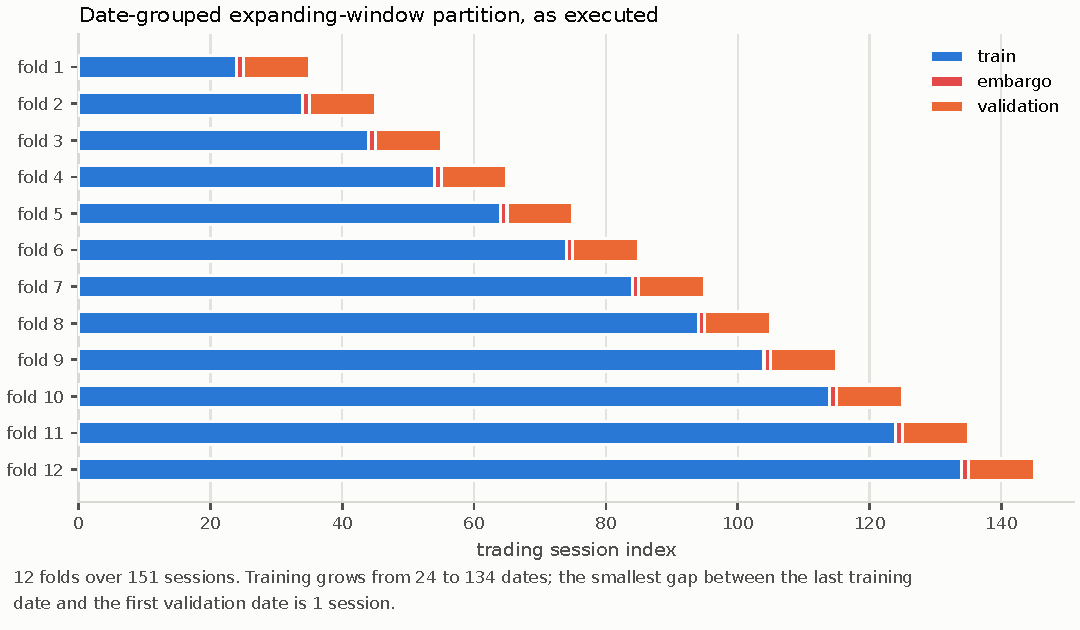
\includegraphics[width=\textwidth]{../docs/figures/fig01_fold_geometry.pdf}
  \caption{The executed date-grouped expanding-window partition. Nothing is
  illustrative: each bar spans the dates the fold really used.}
  \label{fig:folds}
\end{figure}

\subsection{Effective sample size}
\label{sec:dependence}

For $k$ cross-sectional units with average pairwise correlation $\bar\rho$, the
variance of a cross-sectional mean is inflated by
\begin{equation}
\mathrm{VIF} = 1 + (k-1)\bar\rho,
\qquad
n_{\mathrm{eff}} = \frac{n}{\mathrm{VIF}}.
\end{equation}
Rather than apply a correction after the fact, the evaluation changes the unit of
inference: every loss differential is averaged across the tickers present on a
date and all tests run on the resulting one-value-per-session series. Row-level
statistics are computed anyway and reported alongside, so the size of the
inflation is visible rather than argued about. Table~\ref{tab:dependence} and
Figure~\ref{fig:ess} give the realised values.

\input{generated/dependence}

\begin{figure}[!htbp]
  \centering
  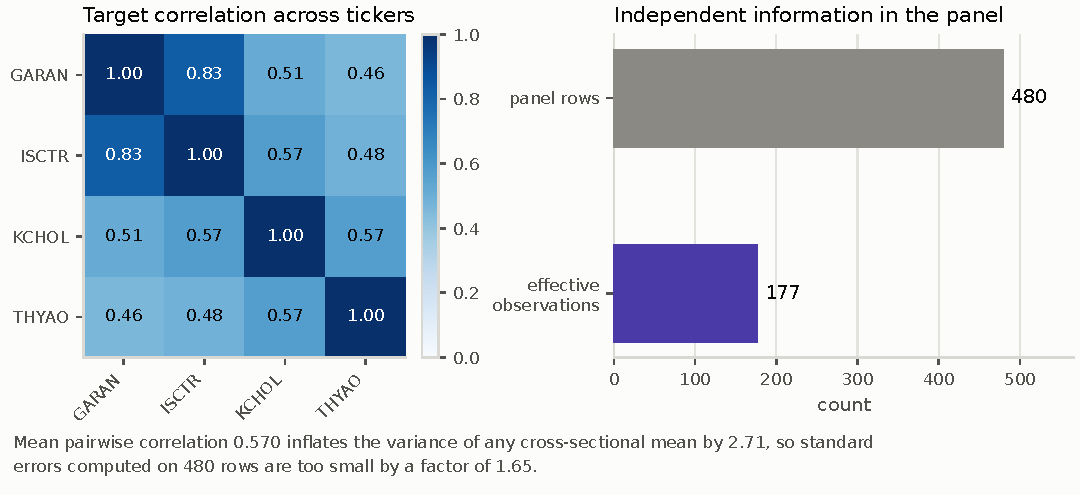
\includegraphics[width=\textwidth]{../docs/figures/fig02_effective_sample_size.pdf}
  \caption{Realised correlation of the executable target across the four tickers,
  and the sample size it implies.}
  \label{fig:ess}
\end{figure}

\subsection{Estimators and metrics}

Seven forecasters share the same panel, target, folds, feature manifest,
evaluation dates and train-only preprocessing: a zero-return null, a
training-fold majority-direction null, a one-session persistence rule, a
same-date cross-sectional mean, a rolling training mean, a regularised logistic
direction model, and a ridge return model that also ranks the portfolio.

The primary accuracy metric is the zero-mean out-of-sample $R^2$,
\begin{equation}
R^2_{0} = 1 - \frac{\sum_{i,t} (r_{i,t} - \hat r_{i,t})^2}{\sum_{i,t} r_{i,t}^2}.
\end{equation}
The sample-mean version is the wrong choice here: its benchmark uses the mean of
the evaluation window, which is not available at prediction time, so it flatters
any model that merely learns the window's drift.

\subsection{Tests}

\textbf{Equal predictive accuracy.} With session-aggregated squared-error
differentials $d_t = L_t(\mathrm{model}) - L_t(\mathrm{null})$,
\begin{equation}
DM = \frac{\bar d}{\sqrt{\hat\Omega / n}},
\qquad
DM^{\ast} = DM \sqrt{\frac{n + 1 - 2h + h(h-1)/n}{n}},
\end{equation}
with $\hat\Omega$ the Bartlett long-run variance and $h=1$, referred to a Student
$t$ distribution on $n-1$ degrees of freedom \citep{diebold1995,harvey1997}. The
sign convention is reported with every test: a \emph{positive} statistic means
the model is worse than the null. Six models are tested against the same null on
the same data, so Holm's step-down procedure \citep{holm1979} controls the
family-wise error rate without assuming independence.

\textbf{Data snooping.} With $Z_{k,t} = L_t(\mathrm{null}) - L_t(\mathrm{model}\;
k)$,
\begin{equation}
V_n = \max_k \sqrt{n}\, \bar Z_k,
\qquad
T_n = \max\!\left[ 0, \; \max_k \frac{\sqrt{n}\, \bar Z_k}{\hat\omega_k} \right],
\end{equation}
whose null distributions come from a stationary bootstrap that resamples every
model on the same index draw, preserving cross-model dependence, with the block
length chosen automatically \citep{white2000,hansen2005,politis1994,politis2004}.

\textbf{Sharpe ratio under search.} For per-period Sharpe $\hat{SR}$ with
skewness $\hat\gamma_3$ and kurtosis $\hat\gamma_4$,
\begin{equation}
\widehat{PSR}(SR^{\ast}) = \Phi\!\left[
\frac{(\hat{SR} - SR^{\ast})\sqrt{n-1}}
{\sqrt{1 - \hat\gamma_3 \hat{SR} + \frac{\hat\gamma_4 - 1}{4}\hat{SR}^2}}
\right],
\end{equation}
and the deflated Sharpe ratio evaluates it at the threshold the best of $N$
skill-free trials would be expected to reach,
\begin{equation}
SR^{\ast}_0 = \sqrt{V[\hat{SR}]}\left[
(1-\gamma)\,\Phi^{-1}\!\left(1 - \tfrac{1}{N}\right)
+ \gamma\,\Phi^{-1}\!\left(1 - \tfrac{1}{Ne}\right)\right],
\end{equation}
with $\gamma$ the Euler--Mascheroni constant \citep{bailey2012,bailey2014dsr}.
Both quantities are per period; substituting an annualised value inflates the
result silently. Lo's autocorrelation-aware annualisation factor
\citep{lo2002} is reported alongside the square-root rule, with lags truncated at
the Newey--West bandwidth \citep{newey1987,newey1994} because 120 sessions cannot
estimate 251 autocorrelations.

\subsection{Portfolio simulation}

Long-only, top-$k$ by predicted return, equal weights, next-open execution at
observed prices, one-session holding. A name is bought only when its predicted
return net of the declared decision-cost assumption is positive. Participation
caps and market impact use a 20-session trailing volume reference whose last
observation is no later than the signal date. The ledger records signals, orders,
fills, positions, cash and costs as separate artifacts and enforces
$E_T = E_0 + \mathrm{PnL}_{\mathrm{gross}} + \mathrm{distributions} -
\mathrm{costs}$. Cost sensitivity reuses the same trading decisions across
multipliers, so only the bill moves.

\section{Results}

\subsection{No fitted model reaches the null}

\input{generated/prediction}
\input{generated/accuracy}

Every fitted model has negative out-of-sample $R^2$ (Table~\ref{tab:prediction}
and Figure~\ref{fig:r2}). Under Holm correction, four of the six are
significantly \emph{worse} than the null and none is better
(Table~\ref{tab:accuracy}); \texttt{logistic} and \texttt{rolling\_mean} are
indistinguishable from it. This is a stronger negative statement than ``no model
beat the benchmark'': several models are reliably worse than predicting zero,
which is what fitting a linear model to a signal-free panel produces.

\begin{figure}[!htbp]
  \centering
  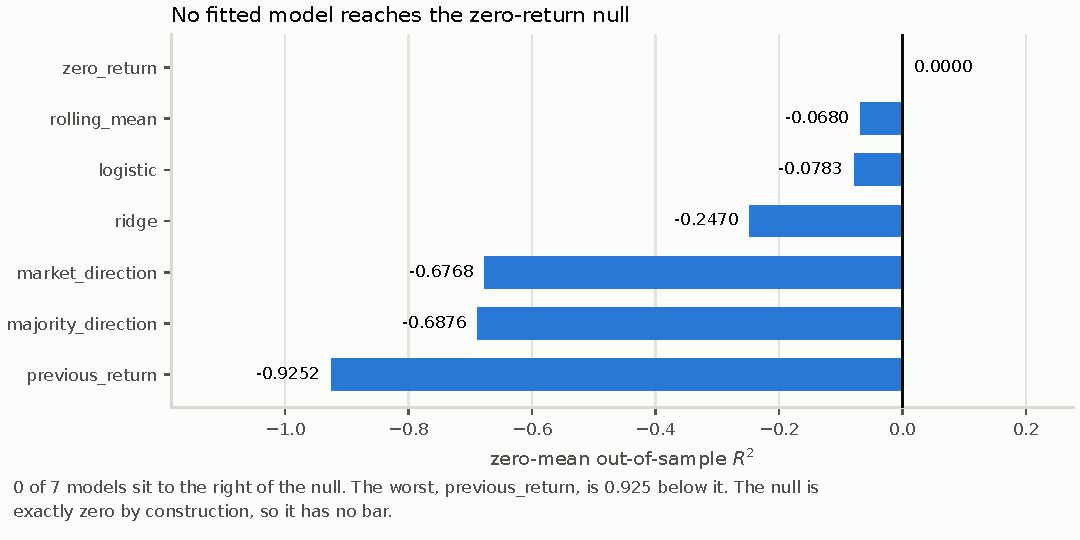
\includegraphics[width=\textwidth]{../docs/figures/fig03_out_of_sample_r_squared.pdf}
  \caption{Zero-mean out-of-sample $R^2$ by model. The null is exactly zero by
  construction and therefore has no bar.}
  \label{fig:r2}
\end{figure}

\begin{figure}[!htbp]
  \centering
  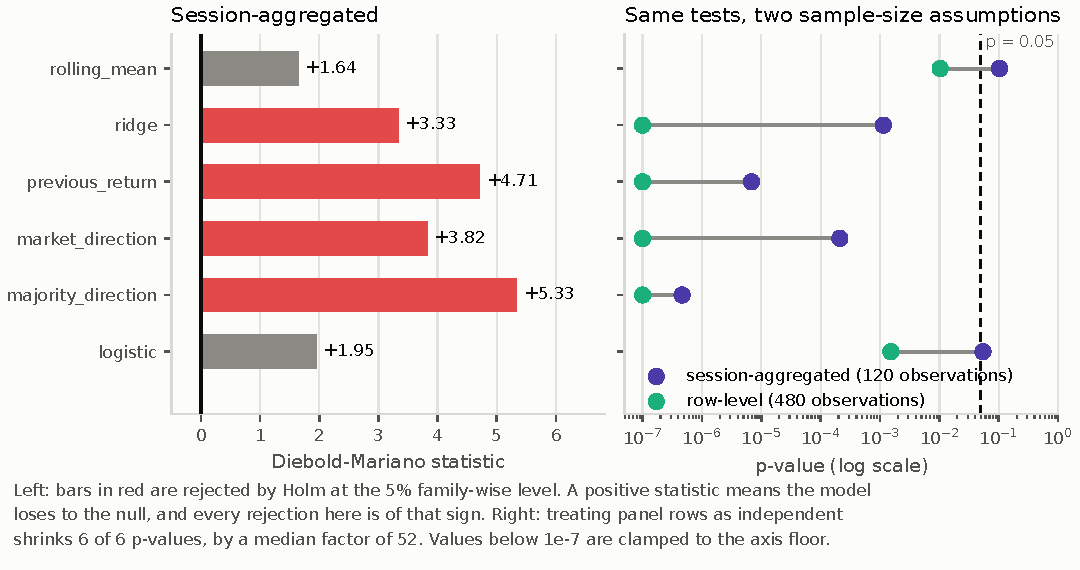
\includegraphics[width=\textwidth]{../docs/figures/fig04_equal_accuracy_tests.pdf}
  \caption{Diebold--Mariano statistics against the zero-return null, and the same
  six tests under two sample-size assumptions. Treating the 480 panel rows as
  independent shrinks every p-value, by a median factor of 52.}
  \label{fig:dm}
\end{figure}

The right panel of Figure~\ref{fig:dm} makes the dependence problem concrete. At
row level \texttt{logistic} reaches $p = 0.0015$; at session level it is $0.0541$
and does not survive correction. Nothing about the data changed, only the claim
about how much of it is independent. The same reversal applies in the other
direction: the four rejections that survive Holm correction are all of the sign
that says the model is worse, so the corrected table contains no discovery at
all.

Directional accuracy deserves a word, because it is the metric this literature
usually leads with. In this window $53.12\%$ of realised targets are
non-positive, so a constant ``down'' predictor attains $53.12\%$ directional
accuracy while carrying no information whatever. That is exactly the figure
\texttt{zero\_return} and \texttt{majority\_direction} reach in
Table~\ref{tab:prediction}, and it is above what \texttt{ridge},
\texttt{logistic} and \texttt{rolling\_mean} manage. Directional accuracy without
its base rate is not interpretable, which is why balanced accuracy is reported
beside it and neither is used as a headline.

\subsection{Nothing survives the search correction}
\label{sec:snooping}

\input{generated/snooping}

\begin{figure}[!htbp]
  \centering
  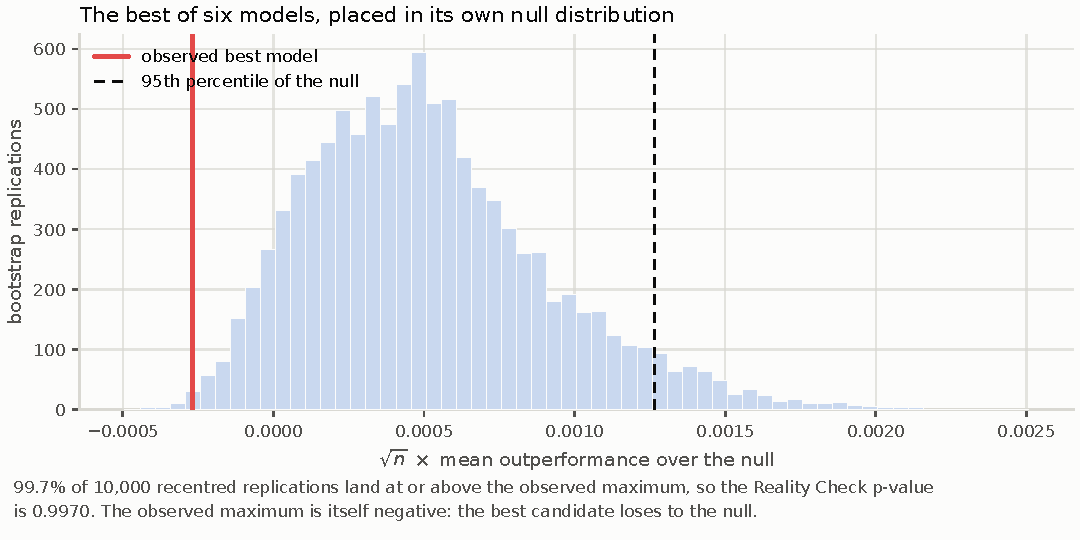
\includegraphics[width=\textwidth]{../docs/figures/fig05_reality_check.pdf}
  \caption{The best of six models placed inside its own bootstrap null
  distribution. The null is centred above zero because it is the distribution of
  a maximum over six candidates: that offset is the data-snooping correction made
  visible. The observed maximum is negative.}
  \label{fig:rc}
\end{figure}

\input{generated/sharpe}
\input{generated/sensitivity}

\begin{figure}[!htbp]
  \centering
  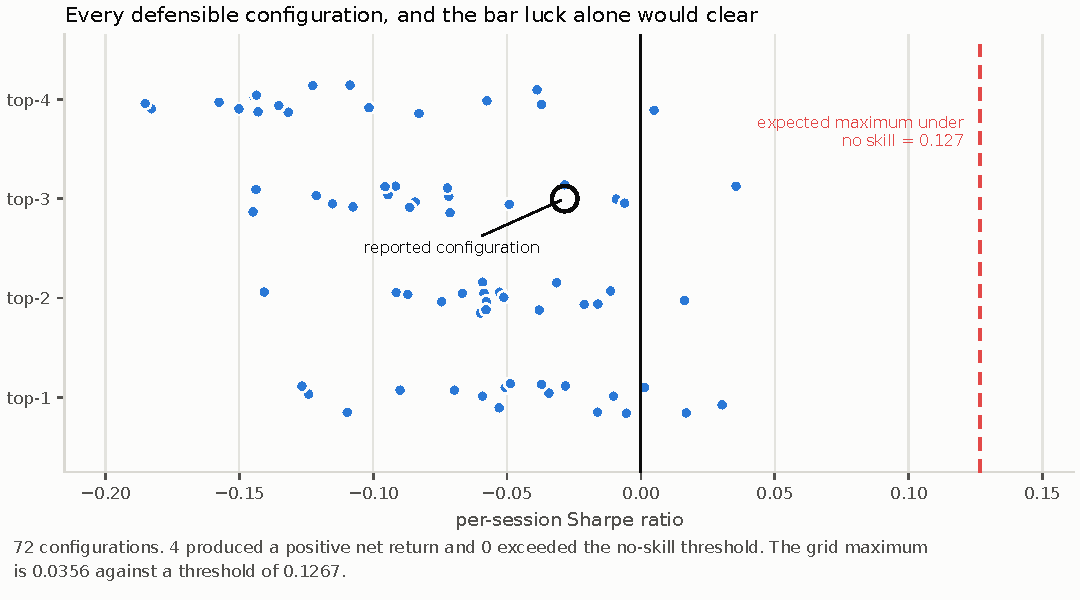
\includegraphics[width=\textwidth]{../docs/figures/fig08_configuration_search.pdf}
  \caption{Every configuration in the grid against the Sharpe ratio that
  skill-free search alone would be expected to produce. The grid maximum does not
  reach the bar luck sets.}
  \label{fig:grid}
\end{figure}

Figure~\ref{fig:rc} is the argument of Section~4.5 in one picture. The bootstrap
null distribution is centred \emph{above} zero because it is the distribution of
a maximum over six candidates; that offset is precisely the data-snooping
correction, made visible. The observed maximum lies to the left of it and is
itself negative, so the best candidate loses to the null before any correction is
applied. Table~\ref{tab:snooping} gives the joint p-values: $0.9970$ for the
Reality Check and $0.6891$ for Hansen's consistent recentring, bracketed by
$0.6891$ and $1.0000$. The joint null is nowhere near rejection.

Table~\ref{tab:sharpe} carries the same message for the portfolio. Session
returns have a kurtosis of $7.2290$, so the normal-theory Sharpe interval
understates tail risk; accounting for the higher moments, the probability that
the true per-session Sharpe exceeds zero is $0.3782$, already below even odds
before any search correction. Deflating by the 72 configurations examined leaves
a deflated Sharpe ratio of $0.0452$.

The grid itself varies the minimum training window, the validation width and
step, the embargo and the portfolio breadth; each point is a complete re-run of
the evaluation, not a re-weighting of a cached result
(Table~\ref{tab:sensitivity}, Figure~\ref{fig:grid}). Only $5.56\%$ of those
configurations produced a positive net return. The reported configuration ranks
16th of 72 by Sharpe ratio, so it is neither cherry-picked nor unusually unlucky,
and the grid maximum of $0.0356$ falls short of the $0.1267$ that the best of 72
skill-free configurations would be expected to reach. The most compact statement
of the result is that across all 72 configurations, the zero-return null attained
the best out-of-sample $R^2$ in 72 of 72.

\subsection{Costs, not signal, decide the outcome}
\label{sec:costs}

\input{generated/portfolio}
\input{generated/costs}

\begin{figure}[!htbp]
  \centering
  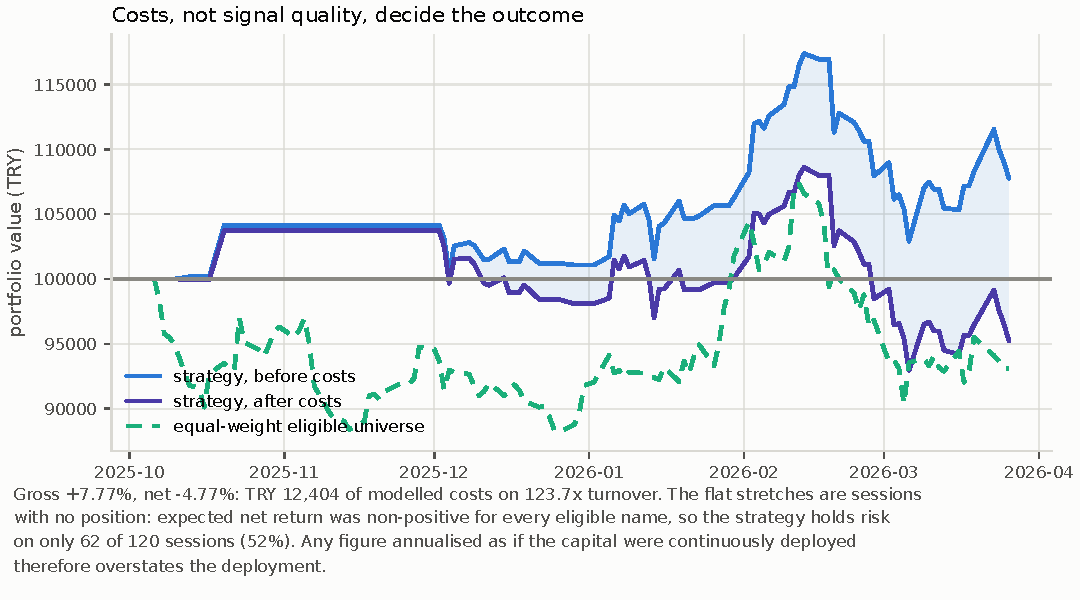
\includegraphics[width=\textwidth]{../docs/figures/fig06_equity_curve.pdf}
  \caption{Gross and net equity against the equal-weight eligible universe. The
  flat stretches are sessions with no position: the strategy holds risk on 62 of
  120 sessions, so annualised figures overstate the deployment.}
  \label{fig:equity}
\end{figure}

\begin{figure}[!htbp]
  \centering
  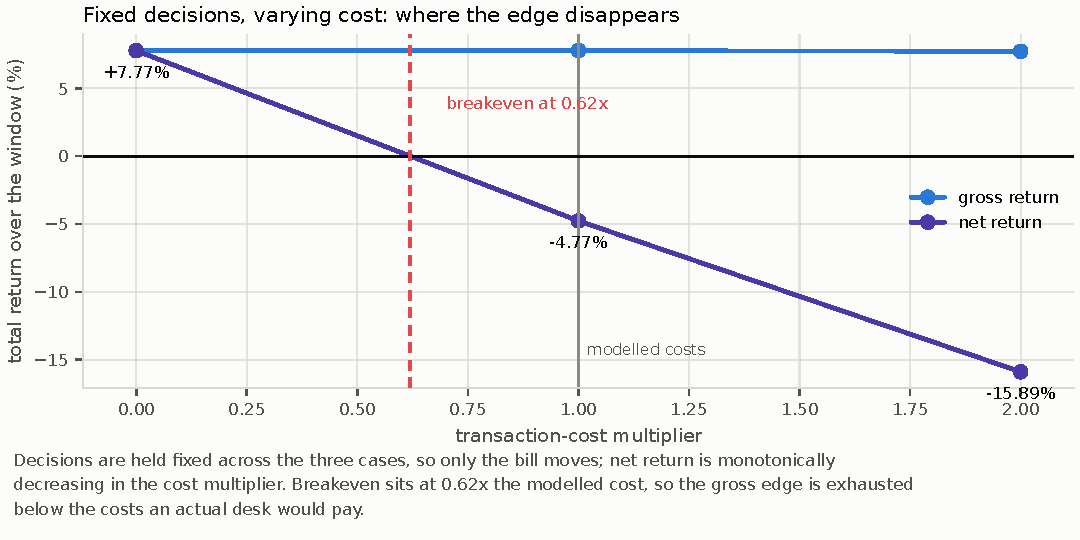
\includegraphics[width=\textwidth]{../docs/figures/fig07_cost_sensitivity.pdf}
  \caption{Fixed trading decisions under three cost multipliers. Breakeven sits
  at $0.62\times$ the modelled schedule.}
  \label{fig:costs}
\end{figure}

The strategy earns a gross return of $7.77\%$ and loses $4.77\%$ of its capital
after costs, on $123.7\times$ turnover and TRY $12{,}404$ of modelled cost
(Table~\ref{tab:portfolio}). Because the trading decisions are held fixed across
the three cost cases, Table~\ref{tab:costs} isolates the bill: net return falls
monotonically, and interpolating between the zero-cost and modelled-cost cases
puts breakeven at $0.62\times$ the modelled schedule, comfortably below what an
actual desk would pay. This reproduces \citet{novymarx2016} at small scale: the
gross edge is real and the net edge is not.

Figure~\ref{fig:equity} shows something the return statistics hide. The flat
stretches are sessions in which no eligible name had a positive expected net
return, so the strategy held nothing; it carries risk on 62 of 120 sessions. Any
figure annualised as though the capital were continuously deployed, including the
annualised return and Sharpe ratio in Table~\ref{tab:portfolio}, therefore
overstates the deployment and is reported only because it is the convention.

\subsection{The conclusion does not depend on the arbitrary choices}

A bootstrap block length is an arbitrary choice, so all seven candidates are
reported rather than one (Table~\ref{tab:blocks}, Figure~\ref{fig:blocks}). Every
interval contains zero and their widths vary by about ten percentage points out
of ninety, so the interval is a statement about the data rather than about the
block length. The automatic Politis--White selection lands at $2.12$ sessions for
the portfolio return series and at $12.26$ for the loss differentials, which is
why the two bootstraps in this paper carry different block lengths.

\input{generated/blocks}

\begin{figure}[!htbp]
  \centering
  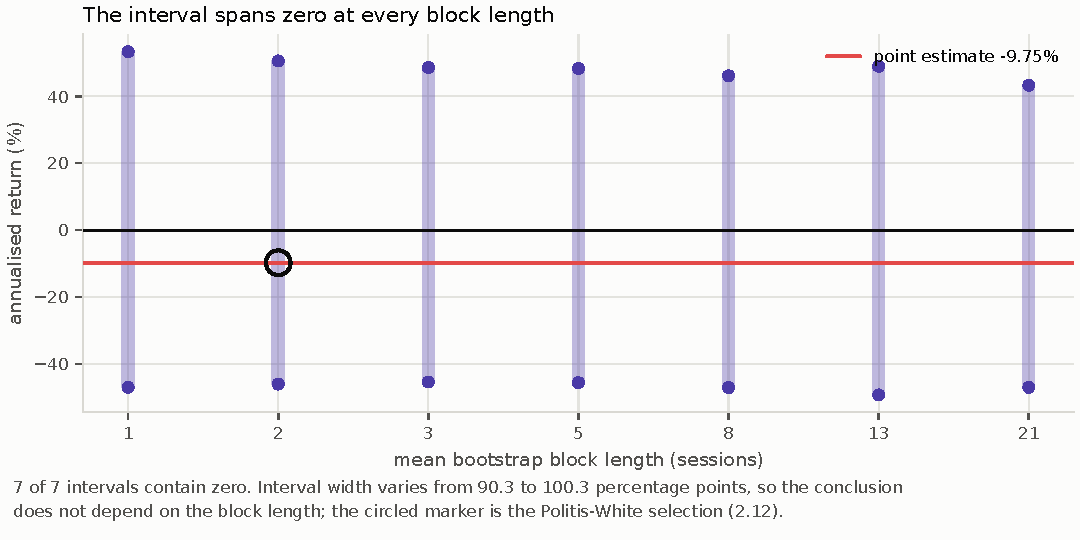
\includegraphics[width=\textwidth]{../docs/figures/fig09_block_length_sensitivity.pdf}
  \caption{The 95\% bootstrap interval for annualised return across seven block
  lengths. Every interval contains zero.}
  \label{fig:blocks}
\end{figure}

\section{Discussion}

On this universe, over this window, at this horizon, scale-normalised price and
volume features carry no out-of-sample information about next-session
open-to-close returns that survives an honest accounting of sample size and
search. The apparatus is not merely failing to reject: several models are
measurably worse than the null, and the family is far from rejection jointly.

This does not mean Borsa Istanbul is efficient, that no short-horizon signal
exists, or that machine learning cannot forecast equity returns. Four stocks over
one year is a small sample. What is strong here is the conditional statement: an
effect large enough to be usable at this horizon on this universe would have
shown up, and it did not.

Two details deserve emphasis. First, a model with no signal does not merely fail
to help; it adds estimation variance to the forecast, which is a pure cost in a
squared-error comparison against a zero forecast. Observing several fitted models
below zero is therefore a consistency check rather than a surprise. Second, the
False Strategy threshold is an \emph{expectation}, not a critical value: a
genuinely skill-free grid exceeds it about half the time, which the accompanying
test suite verifies by simulation. It is reported as a diagnostic, and the
deflated Sharpe ratio, which converts it into a probability, is the actual test.

\section{Limitations}

Four stocks and 120 evaluated sessions are too few for a strong economic
conclusion, and the confidence intervals say so. The universe is a fixed
prototype rather than point-in-time index membership. The committed input
contains no BIST index series, so only cash and an equal-weight
eligible-universe benchmark are reported and no index-relative claim is made.
Sector metadata is unavailable and is reported as unavailable rather than filled
with a placeholder. The strategy holds risk on 62 of 120 sessions, so annualised
figures assume a deployment that did not occur. The search grid is itself a
choice: a different grid would give a different deflation threshold, and the grid
is declared in the run configuration so the choice is auditable. Corporate-action
transition and fail-closed policies are exercised by synthetic tests; the
empirical snapshot contains cash dividends only. Finally, the repository
implements Kalman filters, Ornstein--Uhlenbeck mean reversion, GARCH, HMM
regimes, wavelets, cointegration, Kelly sizing, gradient boosting, stacking,
calibration and neural sequence models, none of which is part of the accepted
experiment; their presence is not evidence of predictive value.

\section{Conclusion}

Seven forecasters were evaluated on a leakage-controlled Borsa Istanbul panel
with an executable target, under tests that account for cross-sectional
dependence, the number of models compared, and the number of configurations
examined. No model beats the zero-return null, four are significantly worse, the
joint data-snooping null is not rejected at any conventional level, and the best
of 72 configurations does not reach the Sharpe ratio that skill-free search alone
would produce. The reported strategy loses money after costs and would lose money
at $0.62\times$ the modelled cost schedule.

The useful output is the apparatus rather than the sign of the result: a target
the backtest can trade, an evaluation whose unit of inference matches the data's
dependence structure, a search that is counted rather than hidden, and a run that
replays byte-for-byte. The next legitimate step is better point-in-time data over
a longer dated universe, not another model family.

\section*{Reproducibility}

Every number in this manuscript is generated from one immutable run bundle by a
tested module and regenerated by \texttt{make paper}. The run replays
byte-for-byte from bundled inputs with \texttt{make reproduce-committed}, and
\texttt{make mutation-check} reintroduces sixteen real defects into the source
and requires the guarding test to fail for each. Code and artifacts:
\url{https://github.com/ITheClixs/BIST-Predictor-advanced}.

\bibliographystyle{unsrtnat}
\bibliography{references}

\appendix

\section{Full configuration grid}

\input{generated/grid_appendix}

\end{document}
